% !TeX program = pdflatex
% Repository-aware engineering guidance for AGENTS.md
% Standalone, pdfLaTeX-compatible report.
\documentclass[11pt,letterpaper]{article}

\usepackage[T1]{fontenc}
\usepackage[utf8]{inputenc}
\usepackage{lmodern}
\usepackage{microtype}
\usepackage[margin=0.88in,headheight=16pt,footskip=28pt]{geometry}
\usepackage[table]{xcolor}
\usepackage{graphicx}
\usepackage{tabularx,booktabs,array,longtable}
\usepackage{enumitem}
\usepackage{titlesec}
\usepackage{fancyhdr}
\usepackage{lastpage}
\usepackage{tikz}
\usetikzlibrary{positioning,arrows.meta,shapes.geometric,fit}
\usepackage[most]{tcolorbox}
\usepackage{listings}
\usepackage{hyperref}
\usepackage{bookmark}
\usepackage{needspace}

% -- Palette -----------------------------------------------------------------
\definecolor{ink}{HTML}{182A3B}
\definecolor{slate}{HTML}{526477}
\definecolor{accent}{HTML}{007B87}
\definecolor{accentdark}{HTML}{005E69}
\definecolor{mist}{HTML}{EAF4F4}
\definecolor{paleblue}{HTML}{EDF2F7}
\definecolor{linegray}{HTML}{D8E1E8}
\definecolor{paper}{HTML}{F8FAFC}
\definecolor{amber}{HTML}{C47B11}

\hypersetup{
  pdftitle={AGENTS.md: Repository-Aware Guidance for AI Coding Agents},
  pdfauthor={Engineering Reference Guide},
  pdfsubject={AGENTS.md, agent instructions, LaTeX repository governance},
  pdfkeywords={AGENTS.md, coding agents, Codex, LaTeX, repository guidelines},
  colorlinks=true,
  linkcolor=accentdark,
  urlcolor=accentdark,
  citecolor=accentdark
}

\setlength{\parindent}{0pt}
\setlength{\parskip}{0.55em}
\setlist[itemize]{topsep=4pt,itemsep=2pt,parsep=0pt,leftmargin=1.45em}
\setlist[enumerate]{topsep=4pt,itemsep=3pt,parsep=0pt,leftmargin=1.6em}
\renewcommand{\arraystretch}{1.25}
\setlength{\emergencystretch}{3em}

\titleformat{\section}{\Large\bfseries\color{ink}}{\thesection}{0.75em}{}[\vspace{2pt}\color{linegray}\titlerule]
\titleformat{\subsection}{\large\bfseries\color{accentdark}}{\thesubsection}{0.65em}{}
\titleformat{\subsubsection}{\normalsize\bfseries\color{ink}}{\thesubsubsection}{0.65em}{}
\titlespacing*{\section}{0pt}{1.55em}{0.75em}
\titlespacing*{\subsection}{0pt}{1.05em}{0.45em}

\pagestyle{fancy}
\fancyhf{}
\fancyhead[L]{\footnotesize\sffamily\color{slate}AGENTS.md / Engineering Reference}
\fancyhead[R]{\footnotesize\sffamily\color{slate}LATEX-DOCS}
\fancyfoot[L]{\footnotesize\sffamily\color{slate}16 November 2026}
\fancyfoot[R]{\footnotesize\sffamily\color{slate}\thepage\ / \pageref{LastPage}}
\renewcommand{\headrulewidth}{0.3pt}
\renewcommand{\footrulewidth}{0pt}

\newtcolorbox{infobox}[1][]{
  enhanced, breakable, colback=mist, colframe=accent!60!white,
  boxrule=0.45pt, arc=1.8mm, left=3.5mm,right=3.5mm,top=2.2mm,bottom=2.2mm,
  borderline west={2.8pt}{0pt}{accent}, #1
}
\newtcolorbox{neutralbox}[1][]{
  enhanced, breakable, colback=paper, colframe=linegray,
  boxrule=0.5pt, arc=1.5mm, left=3.5mm,right=3.5mm,top=2.2mm,bottom=2.2mm,#1
}
\newcommand{\tagpill}[1]{\tcbox[on line,boxrule=0pt,arc=2pt,boxsep=2.5pt,left=6pt,right=6pt,colback=mist,coltext=accentdark]{\sffamily\scriptsize\bfseries #1}}
\newcommand{\pathcode}[1]{\texttt{\detokenize{#1}}}

\lstdefinestyle{agentlisting}{
  basicstyle=\ttfamily\footnotesize,
  backgroundcolor=\color{paper},
  rulecolor=\color{linegray},
  frame=single,
  framesep=7pt,
  columns=fullflexible,
  keepspaces=true,
  breaklines=true,
  breakatwhitespace=true,
  showstringspaces=false,
  numbers=left,
  numberstyle=\tiny\color{slate},
  numbersep=8pt,
  xleftmargin=1.0em,
  framexleftmargin=1.0em,
  aboveskip=9pt,
  belowskip=9pt,
  postbreak=\mbox{\textcolor{accent}{$\hookrightarrow$}\space},
  literate={->}{{$\rightarrow$}}2
}
\lstset{style=agentlisting}

\begin{document}
\pagenumbering{Roman}

% -- Cover -------------------------------------------------------------------
\begin{titlepage}
\thispagestyle{empty}
\vspace*{1.0cm}
{\color{accent}\rule{0.14\linewidth}{5pt}}\\[1.0cm]
{\sffamily\color{accentdark}\large\bfseries TECHNICAL REFERENCE \textbullet\ REPOSITORY GOVERNANCE}\\[0.45cm]
{\sffamily\bfseries\color{ink}\fontsize{32}{37}\selectfont AGENTS.md\\[0.10cm]
Repository-Aware Guidance\\
for AI Coding Agents}\\[0.70cm]
{\color{slate}\Large Open instruction format, agent compatibility, and\\
a deployment blueprint for \texttt{latex-docs}}\\[1.0cm]
\tagpill{REFERENCE GUIDE}\hspace{0.45cm}\tagpill{IMPLEMENTATION BLUEPRINT}\hspace{0.45cm}\tagpill{PDFLATEX COMPATIBLE}

\vfill
\begin{tcolorbox}[colback=ink,colframe=ink,boxrule=0pt,arc=1.5mm,
    left=5mm,right=5mm,top=5mm,bottom=5mm]
{\color{white}\sffamily\large\bfseries Executive premise}\\[3pt]
{\color{white}\normalsize An \texttt{AGENTS.md} file is an operational instruction layer for coding agents. It should \emph{complement}, not duplicate, the human-facing \texttt{README.md}; identify verified commands; and express review, security, and authoring expectations without pretending that prose alone enforces policy.}
\end{tcolorbox}
\vspace{1.0cm}
{\sffamily\color{ink}\bfseries Scope}\quad \texttt{Notoriousjayy/latex-docs}\\[4pt]
{\sffamily\color{slate}Version 1.0 \quad\textbullet\quad 16 November 2026 \quad\textbullet\quad Proposed guidance; no repository changes made}
\end{titlepage}

\tableofcontents
\clearpage
\pagenumbering{arabic}

\section{Executive overview}

\texttt{AGENTS.md} is a simple, open, Markdown-based format that places operating instructions for AI coding agents in a predictable repository location. It typically records project conventions, setup and validation commands, important paths, and expectations for reviewing changes. The official project describes the file as a companion to \texttt{README.md}, not a substitute for conventional documentation.\footnote{Official AGENTS.md guide: \url{https://agents.md/}.}

\begin{infobox}
\textbf{Recommended adoption strategy.} Introduce a concise root-level \texttt{AGENTS.md} in the \texttt{latex-docs} repository. Link to authoritative documentation, make the existing Makefile and tests the validation contract, and add nested instruction files only where local rules differ materially from root guidance.
\end{infobox}

\subsection{What the file should accomplish}
\begin{itemize}
\item \textbf{Reduce ambiguity.} Tell an agent where source-of-truth documents live and which commands are supported.
\item \textbf{Constrain the change surface.} Establish a minimum-change preference, an approval boundary, and evidence requirements.
\item \textbf{Keep checks repeatable.} Identify the tests, LaTeX preflight checks, and document build procedures that should run before review.
\item \textbf{Improve portability.} Offer shared guidance that compatible agents can reuse, while preserving tool-specific configuration when necessary.
\end{itemize}

\subsection{What it does not accomplish}
An \texttt{AGENTS.md} file is \emph{not} a security sandbox, a replacement for branch protection, a guarantee that instructions will be obeyed, or an executable policy engine. Permissions, CI, mandatory review, protected environments, and tool-level approval controls must remain independently enforced.

\section{Instruction files and compatibility}

\subsection{A common baseline, not a universal replacement}
Several AI coding environments recognize \texttt{AGENTS.md}, but instruction lookup, precedence, and fallback behavior differ by tool and version. Existing files such as \texttt{CLAUDE.md}, Cursor rules, or GitHub Copilot instruction files may still be necessary for features or environments not covered by the shared format.

\begin{table}[htbp]
\centering
\small
\caption{Instruction conventions and the role each plays}
\label{tab:formats}
\begin{tabularx}{\textwidth}{@{}p{0.29\textwidth}X@{}}
\toprule
\textbf{Convention} & \textbf{Practical use} \\
\midrule
\texttt{AGENTS.md} & Portable repository instructions; a useful default shared across compatible coding agents. \\
\texttt{CLAUDE.md} & Claude-specific project guidance and features; may need to coexist with or reference shared instructions. \\
\texttt{.cursor/rules/*.mdc} & Cursor-specific rule files, including activation and scope behavior. \\
\texttt{.github/copilot-}\newline\texttt{instructions.md} & GitHub Copilot repository-level customization where applicable. \\
\texttt{AGENTS.override.md} & Codex-specific replacement convention at a given directory level; not part of a universal lookup guarantee. \\
\texttt{\~{}/.codex/AGENTS.md} & Codex user-level guidance, outside the repository and specific to that client. \\
\bottomrule
\end{tabularx}
\end{table}

\textbf{Tooling rule:} verify how each agent discovers and combines instructions before removing existing tool-specific configuration. The list above describes typical use, not a promise of identical behavior across clients.\footnote{Codex guidance: \url{https://learn.chatgpt.com/docs/agent-configuration/agents-md}.}

\subsection{Hierarchy and precedence}
A root \texttt{AGENTS.md} is the simplest portable starting point. Some agents additionally discover nested \texttt{AGENTS.md} files, enabling a broad root instruction set and narrower rules for a directory. Codex documents a specific lookup order including user-level instructions and optional \texttt{AGENTS.override.md} files; these details should not be assumed for every other agent.

\begin{neutralbox}
\textbf{Design principle:} Keep global instructions short and stable. Place exceptions near the code or documents they govern, and avoid conflicting or duplicated requirements across levels.
\end{neutralbox}

\section{Design principles for useful agent guidance}

\begin{enumerate}[label=\textcolor{accentdark}{\bfseries\arabic*.}]
\item \textbf{Be executable.} Name real commands with their prerequisites; avoid generic instructions such as ``test everything'' without a test entry point.
\item \textbf{Link, do not clone.} Reference the repository's Makefile, documentation indexes, and style modules rather than reproducing large or easily stale descriptions.
\item \textbf{Specify boundaries.} Explain what must not be changed implicitly: deployment targets, security gates, generated output, third-party content, and protected branches.
\item \textbf{Require evidence.} Ask agents to distinguish tests run successfully, tests not run, and tests that failed, with concise reasons.
\item \textbf{Keep scope local.} Prefer small changes in the relevant domain and prohibit unrelated renaming or reorganization without explicit authorization.
\item \textbf{Treat instructions as versioned code.} Review changes to agent guidance through pull requests and periodically reconcile them with implementation changes.
\end{enumerate}

\section{Repository assessment: latex-docs}

\textbf{Repository:} \url{https://github.com/Notoriousjayy/latex-docs}

This assessment reflects the repository root, \texttt{README.md}, \texttt{Makefile}, and selected directories inspected on 16 November 2026. No root \texttt{AGENTS.md} was present in that inspection. These observations are a point-in-time design input, not a claim that future commits will preserve the exact layout.

\subsection{Authoritative repository layout}
\begin{table}[htbp]
\centering
\small
\caption{Existing repository structure and intended agent instructions}
\begin{tabularx}{\textwidth}{@{}p{0.28\textwidth}X@{}}
\toprule
\textbf{Path} & \textbf{Responsibility} \\
\midrule
\pathcode{src/} & LaTeX documents organized by engineering or subject domain; canonical content. \\
\pathcode{tooling/} & Python build scripts, LaTeX styles, PlantUML tooling, and manifests. \\
\pathcode{tests/} & Automated validation covering builds, styles, diagrams, and collections. \\
\pathcode{catalog/} & Discovery and taxonomy of documents and templates. \\
\pathcode{.github/workflows/} & CI, reusable build workflows, GitHub Pages publishing, and releases. \\
\pathcode{public/} & Staged generated PDFs, logs, and site output. \\
\pathcode{README.md} & Human-facing repository contract and entry points. \\
\pathcode{Makefile} & Developer-facing, stable build command surface. \\
\bottomrule
\end{tabularx}
\end{table}

The repository explicitly treats LaTeX source as authoritative and generated PDF files as build products. It uses a \textbf{pdfLaTeX-only policy}, semantic style modules under \pathcode{tooling/styles/latex/}, and a shared house style under \pathcode{tooling/latex/}. These contracts are important enough to appear in the root agent instructions.

\subsection{Commands confirmed in the existing Makefile}
\begin{lstlisting}
# Inspect and validate
make help
make list-roots
make list-categories
make preflight
python3 -m unittest discover -s tests
git diff --check

# Build selected or changed documents
make build-category-architecture
make build-changed BASE_REF=<sha> HEAD_REF=<sha>

# Broader build and publication tasks
make build-parallel JOBS=4
make render-plantuml
make plan PLAN_MODE=changed
make publish
\end{lstlisting}

\begin{infobox}
\textbf{Build decision.} For ordinary documentation changes, prefer targeted validation and affected-document builds. Full-corpus builds and publishing are broader operations and should be performed when warranted by the change scope and repository workflow.
\end{infobox}

\section{Proposed agent instruction architecture}

\subsection{Directory-specific instruction plan}
\begin{table}[htbp]
\centering
\small
\caption{Recommended instruction-file rollout}
\label{tab:rollout}
\begin{tabularx}{\textwidth}{@{}p{0.29\textwidth}p{0.14\textwidth}X@{}}
\toprule
\textbf{Proposed file} & \textbf{Priority} & \textbf{Scope of guidance} \\
\midrule
\pathcode{AGENTS.md} & Phase 1 & Source-of-truth rules, safe-change procedure, verification commands, review and security boundaries. \\
\pathcode{src/AGENTS.md} & Phase 2 & LaTeX authoring, metadata, semantic styles, diagrams, domain README and catalog updates. \\
\pathcode{tooling/AGENTS.md} & Phase 2 & Build scripts, renderer contracts, style changes, generated asset integrity. \\
\pathcode{tests/AGENTS.md} & Phase 2 & Regression expectations, unit-test patterns, fixture and negative-test conventions. \\
\pathcode{.github/AGENTS.md} & Phase 3 & GitHub Actions permissions, safe CI changes, Pages and release validation. \\
\bottomrule
\end{tabularx}
\end{table}

\begin{center}
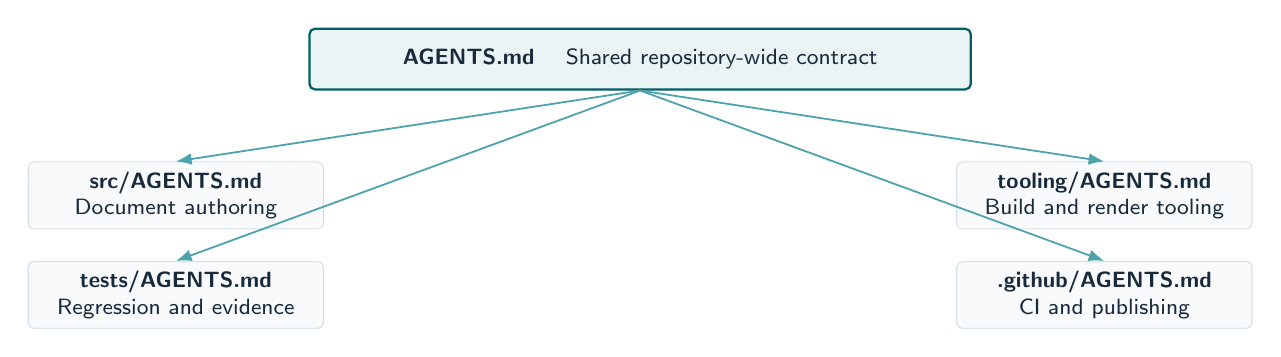
\begin{tikzpicture}[
  node distance=4mm and 6mm,
  every node/.style={font=\sffamily\footnotesize},
  root/.style={draw=accentdark,rounded corners=2pt,fill=mist,text=ink,minimum height=0.77cm,minimum width=8.4cm,align=center,line width=0.8pt},
  child/.style={draw=linegray,rounded corners=2pt,fill=paper,text=ink,minimum height=0.85cm,minimum width=3.75cm,align=center},
  connector/.style={draw=accent!70,-{Latex[length=2mm]},line width=0.65pt}
]
\node[root] (r) {\textbf{AGENTS.md} \quad Shared repository-wide contract};
\node[child,below left=9mm and -2mm of r] (s) {\textbf{src/AGENTS.md}\\Document authoring};
\node[child,below right=9mm and -2mm of r] (t) {\textbf{tooling/AGENTS.md}\\Build and render tooling};
\node[child,below=4mm of s] (u) {\textbf{tests/AGENTS.md}\\Regression and evidence};
\node[child,below=4mm of t] (g) {\textbf{.github/AGENTS.md}\\CI and publishing};
\draw[connector] (r.south) -- (s.north);
\draw[connector] (r.south) -- (t.north);
\draw[connector] (r.south) -- (u.north);
\draw[connector] (r.south) -- (g.north);
\end{tikzpicture}
\end{center}

The diagram is a \emph{logical instruction hierarchy}, not a claim that every agent loads all nested files on every task. Actual scope resolution depends on the agent and the files being edited.

\subsection{Rules for nested guidance}
\begin{itemize}
\item Add a nested file only after a recurring domain-specific requirement has been identified.
\item Avoid copying root-level commands into every subdirectory.
\item Reference exact files and commands that already exist in the repository.
\item Do not create contradictory permissions or imply that Markdown instructions override CI security rules.
\end{itemize}

\clearpage
\section{Proposed root AGENTS.md template}

The following template is ready to copy into a new root-level \texttt{AGENTS.md}. It emphasizes existing contracts and avoids claiming checks were performed before an agent actually runs them.

\begin{lstlisting}
# AGENTS.md

## Repository purpose
This repository is a source-controlled LaTeX engineering
and learning documentation library. LaTeX source is
canonical; generated PDFs are build products.

## Read before changing anything
1. Read README.md and the closest domain README.
2. Inspect existing source, templates, and relevant tests.
3. Reuse the current directory taxonomy and tooling.
4. Prefer minimal, scoped changes to unrelated refactors.
5. Explain assumptions when repository evidence is incomplete.

## Repository map
- src/: Authoritative LaTeX source, organized by domain.
- tooling/: Build helpers, styles, diagrams, and manifests.
- tests/: Automated tests and regression coverage.
- catalog/: Discovery catalogs and template inventories.
- .github/workflows/: CI, Pages, and release automation.
- public/: Generated PDFs, logs, and site artifacts.

## Authoring contract
- Use pdfLaTeX-compatible source; obey the preflight policy.
- Reuse the appropriate semantic LaTeX style module under
  tooling/styles/latex/ and the shared house style.
- Use established metadata, naming, and document structure.
- Prefer lowercase kebab-case for new source filenames.
- Keep editable diagram sources under version control.
- Update the nearest README or catalog entry when required.
- Distinguish proposals and blank forms from approved
  decisions, operational evidence, or certification.

## Verification commands
Run the checks applicable to the files you change:

    git diff --check
    python3 -m unittest discover -s tests
    make preflight

For document changes, build the affected roots or category.
Use Makefile targets and tooling/scripts/latex_build.py;
do not invent an alternative build workflow.

Examples:

    make help
    make list-roots
    make build-category-architecture
    make build-changed BASE_REF=<sha> HEAD_REF=<sha>

For PlantUML changes, validate source and rendered output;
use `make render-plantuml` when appropriate.

## Security and publication boundaries
- This repository is public: do not add secrets, personal
  data, confidential records, or unlicensed third-party work.
- Do not bypass branch protection or CI/security checks.
- Do not change publishing, release, or deployment behavior
  without explicit authorization.
- Do not treat generated PDFs as canonical editing targets.
- Do not claim verification passed unless it was run.

## Pull request and completion expectations
- Use a dedicated branch for changes when applicable.
- Summarize changed paths, rationale, and affected artifacts.
- Report commands run and their observed results.
- Identify skipped checks and unresolved risks explicitly.
- Do not merge, release, or deploy without authorization.
\end{lstlisting}

\begin{neutralbox}
\textbf{Operational note.} This is a proposed instruction file, not an action performed on GitHub. Reconcile it with the current branch and any team-specific review requirements before committing.
\end{neutralbox}

\section{Review, validation, and rollout}

\subsection{Implementation sequence}
\begin{enumerate}[label=\textbf{Phase \arabic*:},leftmargin=2.1cm]
\item \textbf{Introduce the root contract.} Add the proposed root \texttt{AGENTS.md} on a dedicated branch, then compare every path and command against the repository's current state.
\item \textbf{Exercise agent discovery.} Ask each target coding agent to identify the instructions it loaded and the expected checks for a small documentation change. Capture differences in behavior; avoid assuming identical precedence.
\item \textbf{Validate representative changes.} Test one LaTeX document edit and, separately, one tooling or test change. Check whether the agent follows source-of-truth rules and reports actual verification evidence.
\item \textbf{Refine only where needed.} Add nested instructions for \texttt{src/}, \texttt{tooling/}, or other subtrees only when observed gaps warrant them.
\item \textbf{Govern revisions.} Review instruction files like code, with an owner, review history, and periodic reconciliation with build/CI changes.
\end{enumerate}

\subsection{Acceptance criteria}
\begin{table}[htbp]
\small
\centering
\caption{Minimum completion criteria for the first pull request}
\begin{tabularx}{\textwidth}{@{}p{0.32\textwidth}X@{}}
\toprule
\textbf{Criterion} & \textbf{Evidence expected} \\
\midrule
Valid repository references & Every mentioned path and command exists in the PR's target branch. \\
Instruction discovery & At least one target agent can describe the root instruction contract accurately. \\
Build policy aligned & The template specifies pdfLaTeX and the existing Makefile rather than a parallel build system. \\
Review boundaries explicit & Merge, deployment, release, and security gate bypasses remain approval-controlled. \\
Verification reported & Pull request shows commands run, outcomes, and any checks that were not executed. \\
No accidental publication & No sensitive source data or unintended generated artifacts are introduced. \\
\bottomrule
\end{tabularx}
\end{table}

\subsection{A concise pull request description}
\begin{neutralbox}
\textbf{Title:} Add repository-aware AGENTS.md guidance\\[3pt]
\textbf{Change:} Introduces a root instruction contract for AI coding agents, grounded in existing LaTeX style, testing, build, and publication workflows.\\[3pt]
\textbf{Validation:} List actual commands executed and their outputs.\\[3pt]
\textbf{Risk:} Documentation-only guidance. No branch protection, CI permission, or deployment settings are changed by this proposal.
\end{neutralbox}

\section{Further reading and source register}

\begin{enumerate}[label={\bfseries [\arabic*]},leftmargin=2.2em,itemsep=7pt]
\item \textbf{AGENTS.md official guide.} Format overview, rationale, and examples.\\
\url{https://agents.md/}
\item \textbf{AGENTS.md project repository.} Open project and community examples.\\
\url{https://github.com/agentsmd/agents.md}
\item \textbf{OpenAI Codex: custom instructions with AGENTS.md.} Codex-specific file discovery, overrides, and testing.\\
\url{https://learn.chatgpt.com/docs/agent-configuration/agents-md}
\item \textbf{latex-docs repository.} Source organization and implementation context.\\
\url{https://github.com/Notoriousjayy/latex-docs}
\item \textbf{latex-docs README and Makefile.} The human-facing repository contract and supported build commands.\\
\url{https://github.com/Notoriousjayy/latex-docs/blob/main/README.md}\\
\url{https://github.com/Notoriousjayy/latex-docs/blob/main/Makefile}
\end{enumerate}

\vfill
\begin{infobox}
\textbf{Final recommendation.} Start with one short, reviewed, root-level \texttt{AGENTS.md}. Keep the README and source files authoritative, preserve tool-specific configurations when needed, and require independent CI/security enforcement for anything that matters operationally.
\end{infobox}

\end{document}